%Préambule du document :
\documentclass[11pt]{article}
\usepackage[utf8]{inputenc}
\usepackage[french]{babel}
\usepackage{amsmath}
\usepackage{tikz}

%Corps du document :
\begin{document}
  \center 
\includegraphics[width=8cm]{logo.png}

\begin{center}
\textsc{\Large M1 Informatique - Projet ANDROIDE}\\[0.5cm]
\textsc{\Large  Carnet de bord }\\[0.5cm]
\textbf{Robotique adaptative en essaim: effet de l'environnement sur l'apprentissage de stratégies collectives} \\[3cm]
\end{center}


\begin{center}
Roza Amokrane\\[0.3cm]
Nabila Ould Belkacem\\[0.8cm]
\textbf{Encadrant:}\\
Nicolas Bredeche \\[0.4cm]
\end{center}


\newpage
\tableofcontents
\newpage

\begin{flushleft}
\section{Introduction}
 Embodied Evolutionary Robotics (EER) est la conception d’algorithmes distribués en ligne implémentés  sur un groupe de robots .C’est une approche automatisée pour l’apprentissage de la spécialisation dans un essaim de comportements permettant d'accélérer l’apprentissage grâce à l’échange d’informations entre les robots  .Pour étudier l'évolution  de cette spécialisation,on dispose de deux ressources dans un environnement où les agents doivent se déplacer pour fourrager ces ressources afin de survivre, ils doivent être capable de synthétiser une  ressource en énergie qui dépend de  leurs génomes.On suppose que chaque agent est capable d’envoyer son propre génome à ses voisins .Pour que  toute la population survive il faut  que la moitié des agents se spécialisent dans une ressource et la moitié dans une autre .
   Pour cela, l’objectif de ce projet consiste dans un premier temps à faire une étude des différents algorithmes de sélection de génome quand les agents apprennent indépendamment , Ensuite on s'intéressera  à l'apprentissage de la coopération, enfin comparer entre les deux méthodes.

\section{Les mots clés retenus}

 \begin{itemize} \item Ressource   \item Graphe  \item Agent\item Génome \item Fitness   \item Algorithme de sélection de génome  \item Fitness-prop \item Rank-prop  \item VaNILLA-ELITIST  \item VaNILLA-NOFITNESS 
  \end{itemize} 
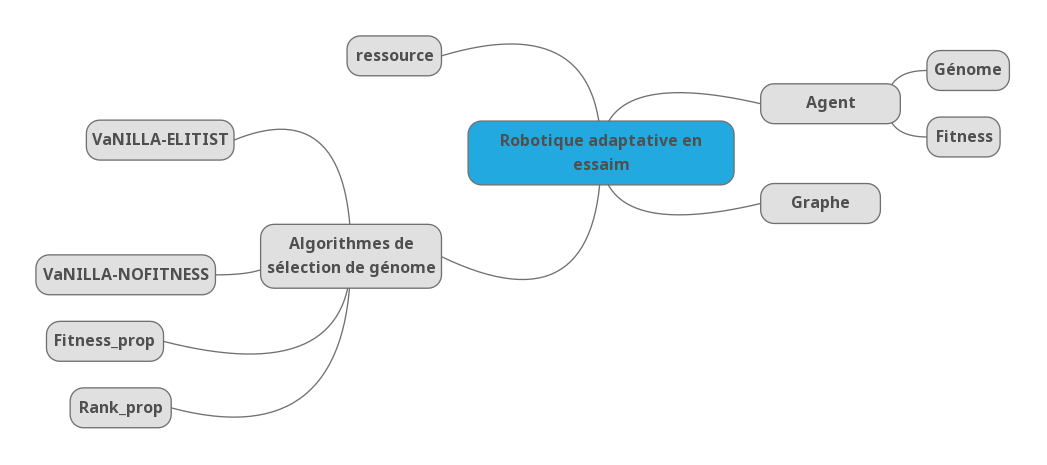
\includegraphics[scale=0.4]{carte.png} 

\section{Descriptif de la recherche documentaire}


\section{Bibliographie produite dans le cadre du projet}
\end{flushleft}
\end{document}
